\documentclass{article}\usepackage[]{graphicx}\usepackage[]{color}
%% maxwidth is the original width if it is less than linewidth
%% otherwise use linewidth (to make sure the graphics do not exceed the margin)
\makeatletter
\def\maxwidth{ %
  \ifdim\Gin@nat@width>\linewidth
    \linewidth
  \else
    \Gin@nat@width
  \fi
}
\makeatother

\definecolor{fgcolor}{rgb}{0.345, 0.345, 0.345}
\newcommand{\hlnum}[1]{\textcolor[rgb]{0.686,0.059,0.569}{#1}}%
\newcommand{\hlstr}[1]{\textcolor[rgb]{0.192,0.494,0.8}{#1}}%
\newcommand{\hlcom}[1]{\textcolor[rgb]{0.678,0.584,0.686}{\textit{#1}}}%
\newcommand{\hlopt}[1]{\textcolor[rgb]{0,0,0}{#1}}%
\newcommand{\hlstd}[1]{\textcolor[rgb]{0.345,0.345,0.345}{#1}}%
\newcommand{\hlkwa}[1]{\textcolor[rgb]{0.161,0.373,0.58}{\textbf{#1}}}%
\newcommand{\hlkwb}[1]{\textcolor[rgb]{0.69,0.353,0.396}{#1}}%
\newcommand{\hlkwc}[1]{\textcolor[rgb]{0.333,0.667,0.333}{#1}}%
\newcommand{\hlkwd}[1]{\textcolor[rgb]{0.737,0.353,0.396}{\textbf{#1}}}%
\let\hlipl\hlkwb

\usepackage{framed}
\makeatletter
\newenvironment{kframe}{%
 \def\at@end@of@kframe{}%
 \ifinner\ifhmode%
  \def\at@end@of@kframe{\end{minipage}}%
  \begin{minipage}{\columnwidth}%
 \fi\fi%
 \def\FrameCommand##1{\hskip\@totalleftmargin \hskip-\fboxsep
 \colorbox{shadecolor}{##1}\hskip-\fboxsep
     % There is no \\@totalrightmargin, so:
     \hskip-\linewidth \hskip-\@totalleftmargin \hskip\columnwidth}%
 \MakeFramed {\advance\hsize-\width
   \@totalleftmargin\z@ \linewidth\hsize
   \@setminipage}}%
 {\par\unskip\endMakeFramed%
 \at@end@of@kframe}
\makeatother

\definecolor{shadecolor}{rgb}{.97, .97, .97}
\definecolor{messagecolor}{rgb}{0, 0, 0}
\definecolor{warningcolor}{rgb}{1, 0, 1}
\definecolor{errorcolor}{rgb}{1, 0, 0}
\newenvironment{knitrout}{}{} % an empty environment to be redefined in TeX

\usepackage{alltt}
\usepackage{natbib}



\IfFileExists{upquote.sty}{\usepackage{upquote}}{}
\begin{document}

\title{Peter Pan Wordcloud}
\author{Tiffany Gonzalez}
\maketitle

\begin{abstract}
Sir James Matthew Barrie is a Scottish novelist and playwright. He is best known for creating the play, in which later became a famously known Disney movie, Peter Pan. Peter Pan is about an ageless boy and Tinkerbell, who is a fairy and companion to Peter Pan. These two have many adventures in the fantasy place, Neverland. This is the perfect playwright for Halloween because it is the time to dress up as fictional or non-fictional characters \citep{Barrie}. In this article, we will be using Sir J.M. Barrie's famous playwright 'Peter Pan or The Boy Who Wouldn't Grow Up' to create a wordcloud.\footnote{A wordcloud will be later defined as the article continues} Let's bring in all of the packages we will be working with in this article.

\begin{knitrout}
\definecolor{shadecolor}{rgb}{0.969, 0.969, 0.969}\color{fgcolor}\begin{kframe}
\begin{alltt}
\hlkwd{library}\hlstd{(dplyr)}
\hlkwd{library}\hlstd{(tm)}
\hlkwd{library}\hlstd{(tidytext)}
\hlkwd{library}\hlstd{(wordcloud)}
\hlkwd{library}\hlstd{(stringr)}
\hlkwd{library}\hlstd{(gutenbergr)}
\hlkwd{library}\hlstd{(knitr)}
\end{alltt}
\end{kframe}
\end{knitrout}


\end{abstract}

\section{The Gutenbergr Package}
There is a package within R, gutenbergr, that gives access to domain works in the Project Gutenberg collection. We have this package installed above. As mentioned previously, we will be focusing on just the book of Peter Pan. To find the book, including Peter Pan, we can run the following code:  To just work with one work, out of all the works, you may call the following function and store the result as follows:

\begin{knitrout}
\definecolor{shadecolor}{rgb}{0.969, 0.969, 0.969}\color{fgcolor}\begin{kframe}
\begin{alltt}
\hlkwd{library}\hlstd{(gutenbergr)}
\hlkwd{library}\hlstd{(stringr)}
\hlkwd{gutenberg_works}\hlstd{(}\hlkwd{str_detect}\hlstd{(title,}\hlstr{'Peter Pan'}\hlstd{))}
\end{alltt}
\begin{verbatim}
## # A tibble: 3 x 8
##   gutenberg_id
##          <int>
## 1         1332
## 2        24012
## 3        39755
## # ... with 7 more variables: title <chr>, author <chr>,
## #   gutenberg_author_id <int>, language <chr>, gutenberg_bookshelf <chr>,
## #   rights <chr>, has_text <lgl>
\end{verbatim}
\end{kframe}
\end{knitrout}

When this code is run, the output gives more than one Peter Pan book. However we know the author is J.M. Barrie, so we can use his gutenberg\_ID number, and store the result:

\begin{knitrout}
\definecolor{shadecolor}{rgb}{0.969, 0.969, 0.969}\color{fgcolor}\begin{kframe}
\begin{alltt}
\hlkwd{library}\hlstd{(gutenbergr)}
\hlstd{peter_pan}\hlkwb{<-}\hlkwd{gutenberg_download}\hlstd{(}\hlnum{39755}\hlstd{)}
\end{alltt}


{\ttfamily\noindent\itshape\color{messagecolor}{\#\# Determining mirror for Project Gutenberg from http://www.gutenberg.org/robot/harvest}}

{\ttfamily\noindent\itshape\color{messagecolor}{\#\# Using mirror http://aleph.gutenberg.org}}\end{kframe}
\end{knitrout}

\section{The Wordcloud}
To make the wordcloud, we first have to break up the lines in the book into words. We can use a function from the tidytext package for this. We can run the following code, and store it into words\_df:

\begin{knitrout}
\definecolor{shadecolor}{rgb}{0.969, 0.969, 0.969}\color{fgcolor}\begin{kframe}
\begin{alltt}
\hlkwd{library}\hlstd{(tidytext)}
\hlstd{words_df}\hlkwb{<-}\hlstd{peter_pan}\hlopt
  \hlkwd{unnest_tokens}\hlstd{(word,text)}

\hlstd{words_df}
\end{alltt}
\begin{verbatim}
## # A tibble: 9,479 x 2
##    gutenberg_id         word
##           <int>        <chr>
##  1        39755 illustration
##  2        39755         with
##  3        39755          the
##  4        39755       spring
##  5        39755        comes
##  6        39755        wendy
##  7        39755          the
##  8        39755        story
##  9        39755           of
## 10        39755        peter
## # ... with 9,469 more rows
\end{verbatim}
\end{kframe}
\end{knitrout}

But within the column of words, we have common, unimportant words such as `the` `a` `was`... These words are referred to as stop words. We can remove these, with the stop\_words data frame and dplyr:

\begin{knitrout}
\definecolor{shadecolor}{rgb}{0.969, 0.969, 0.969}\color{fgcolor}\begin{kframe}
\begin{alltt}
\hlstd{words_df}\hlkwb{<-}\hlstd{words_df}\hlopt
  \hlkwd{filter}\hlstd{(}\hlopt{!}\hlstd{word} \hlopt \hlstd{stop_words}\hlopt{$}\hlstd{word)}

\hlstd{words_df}
\end{alltt}
\begin{verbatim}
## # A tibble: 3,571 x 2
##    gutenberg_id         word
##           <int>        <chr>
##  1        39755 illustration
##  2        39755       spring
##  3        39755        wendy
##  4        39755        story
##  5        39755        peter
##  6        39755          pan
##  7        39755       retold
##  8        39755        fairy
##  9        39755         play
## 10        39755          sir
## # ... with 3,561 more rows
\end{verbatim}
\end{kframe}
\end{knitrout}

A wordcloud is a picture composed of words, in which the size of each word is based off of its frequency.Therefore, we need to calculate the frequencies of the the words in our dataframe. Again, we can use standard dplyr techniques for this:

\begin{knitrout}
\definecolor{shadecolor}{rgb}{0.969, 0.969, 0.969}\color{fgcolor}\begin{kframe}
\begin{alltt}
\hlkwd{library}\hlstd{(dplyr)}
\hlstd{word_freq}\hlkwb{<-}\hlstd{words_df}\hlopt
  \hlkwd{group_by}\hlstd{(word)}\hlopt
  \hlkwd{summarize}\hlstd{(}\hlkwc{count}\hlstd{=}\hlkwd{n}\hlstd{())}

\hlstd{word_freq}
\end{alltt}
\begin{verbatim}
## # A tibble: 1,541 x 2
##          word count
##         <chr> <int>
##  1    _colour     8
##  2    _first_     1
##  3     _hear_     1
##  4      _his_     1
##  5        _i_     1
##  6     _kiss_     1
##  7     _like_     1
##  8       _me_     1
##  9 _thimbles_     1
## 10          1     2
## # ... with 1,531 more rows
\end{verbatim}
\end{kframe}
\end{knitrout}

It's time to create the final product... The Wordcloud!

\begin{knitrout}
\definecolor{shadecolor}{rgb}{0.969, 0.969, 0.969}\color{fgcolor}\begin{kframe}
\begin{alltt}
\hlkwd{library}\hlstd{(wordcloud)}
\hlkwd{wordcloud}\hlstd{(word_freq}\hlopt{$}\hlstd{word,word_freq}\hlopt{$}\hlstd{count,}\hlkwc{min.freq}\hlstd{=}\hlnum{5}\hlstd{)}
\end{alltt}
\end{kframe}
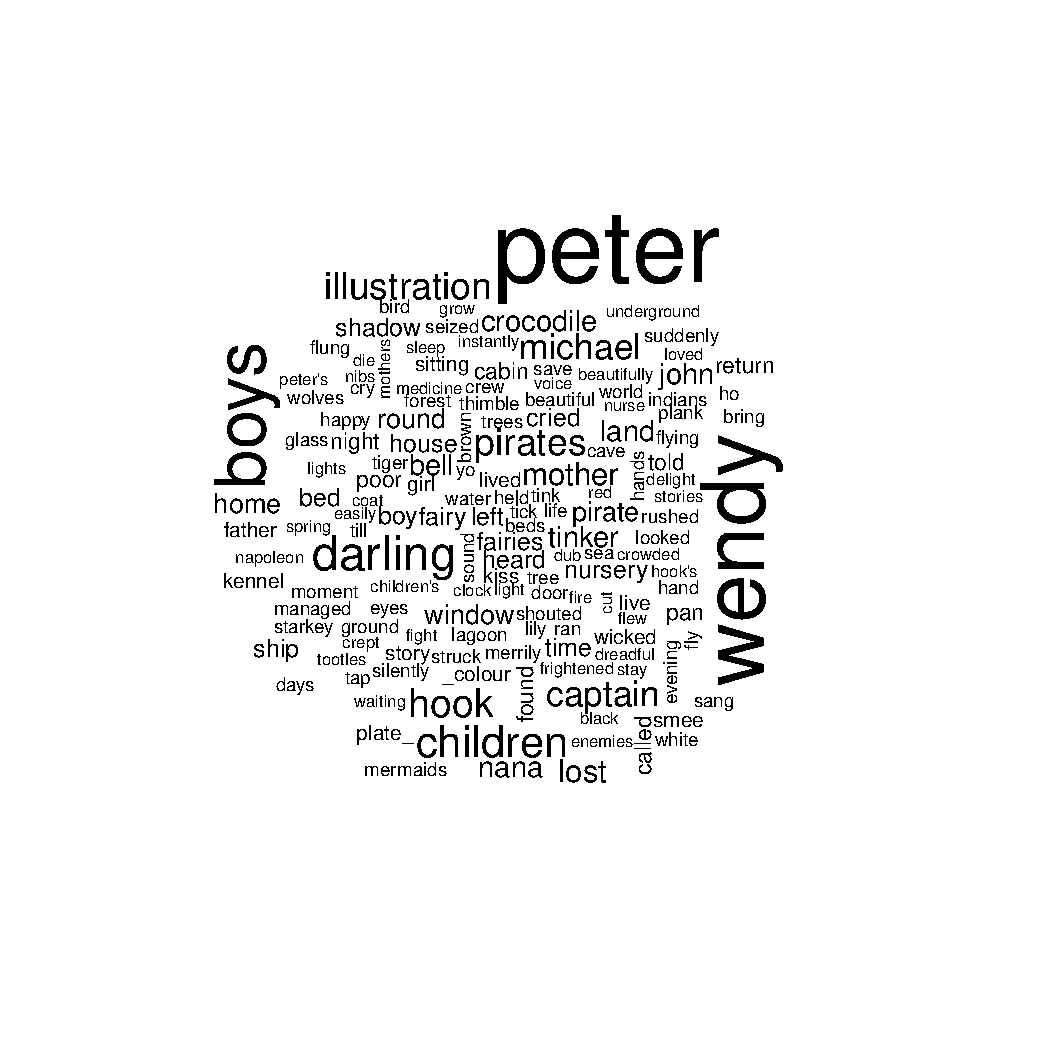
\includegraphics[width=\maxwidth]{figure/unnamed-chunk-8-1} 

\end{knitrout}

\bibliographystyle{apa}
\bibliography{article,packages}
\nocite{*}


\end{document}
